\section{05.11.2014 - Oscillatore a ponte di Wien}

In questa esperienza construiremo un circuito oscillante detto \textit{oscillatore a ponte di Wien} ed effettueremo una pole-zero compensation di una sonda per oscilloscopio.

\subsection*{Strumenti e materiali}

%\begin{figure}[htc]
\begin{itemize} [noitemsep]
	%\item Generatore di forme d'onta Agilent 33120A con range di frequenza da \SI{100}{\micro\hertz} a \SI{15}{\mega\hertz};
	\item Oscilloscopio Agilent DSO-X 2002A (bandwidth \SI{70}{\mega\hertz}, sample rate \num{2} GSa/s);%\newline
%	\begin{minipage}{0.65\textwidth}
%		\vspace{0.4mm}
%%		\begin{itemize} [noitemsep]
%%		\item Oscilloscopio Agilent DSO-X 2002A (bandwidth \SI{70}{\mega\hertz}, sample rate \num{2} GSa/s);
		\item Generatore di tensione continua Agilent E3631A (max $\pm \, \SI{25}{\volt}$ o $\pm \, \SI{6}{\volt}$);
%%		\item Generatore di forme d'onta Agilent 33120A con range di frequenza da \SI{100}{\micro\hertz} a \SI{15}{\mega\hertz};
		\item Multimetro Agilent 34410A a sei cifre e mezza;
		\item Amplificatore operazionale $\mu$A741;
		\item Una lampadina a filamento;
		\item Resistenze e capacità di vari valori;
		%\item Trimmer multigiro da \SI{10}{\kilo\ohm} e \SI{1}{\kilo\ohm};
		\item Breadboard e cablaggi vari.
		\item Una sonda compensata
%%		\end{itemize}
%	\end{minipage}
%	\begin{minipage}{0.3\textwidth}
%			\centering
%			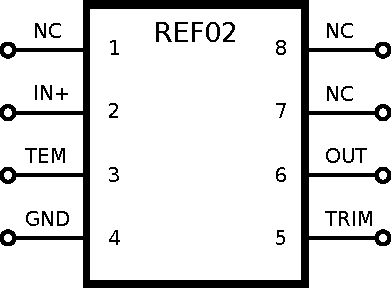
\includegraphics[width=3.5cm]{../E06/latex/REF02.pdf}
%			\caption{Piedinatura dell'integrato\newline REF02.}
%			\label{cir6:REF02}
%	\end{minipage}
\end{itemize}
%\end{figure}
%\vspace{-.8cm}

\begin{wrapfigure}[15]{r}{0.45\textwidth}
\centering
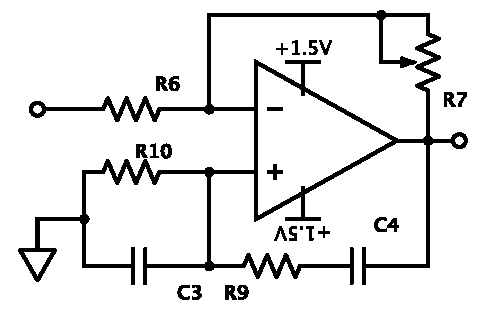
\includegraphics[width=.35\textwidth]{../E08/latex/osc.pdf}
\caption{Schema dell'oscillatore a ponte di Wien senza regolazione del guadagno.}
\label{cir8:without_lamp}
\end{wrapfigure}

\subsection{Oscillatore a ponte di Wien}

L'idea alla base dell'oscillatore a ponte di Wien è quella di sfruttare la selezione in frequenza di un filtro passa banda - il ponte di Wien - caratterizzato da avere il massimo guadagno per una determinata frequenza $f_0$.

All'accensione dell'alimentazione del circuito si crea una forma d'onda quadra che contiene tutte le frequenze e pertanto anche $f_0$ (un'onda quadra puù essere ottenuta tramite serie di Fourier).

Dunque, se riusciamo a stabilizzare il circuito, ovvero evitare che nel tempo o si smorzi o vada in saturazione, avremo una oscillazione alla frequenza $f_0$ e con ampiezza costante. Dovremo dunque imporre un guadagno complessivo unitario.


%Ciò significa che, imponendo unitario il guadagno massimo del circuito, si otterrà un circuito che oscilla con ampiezza costante a $f_0$, con l'ampiezza data dall'ampiezza iniziale.

Lo schema in Figura \ref{cir8:without_lamp} presenta il circuito con amplificazione massima unitaria.
Come si può vedere esso è composto da un opamp con due rami di retroazione negativa e positiva.
Il ramo di feedback positivo è dato dal ponte di Wien mentre quello negativo è composto da un partitore resistivo.

Analizzando il circuito per $\omega_0=2\pi f_0=\frac{1}{RC}$ ($s=\frac{j}{RC}$) otteniamo dai due partitori:

\begin{equation}
  \begin{array}{lr}
	V^+_{f_0} = \frac{Z_{//}}{Z_1 + Z_{//}}V_{out} = \frac{1}{3}V_{out}\\
	V^-_{f_0} = \frac{R_1}{R_1+R_2}V_{out}
  \end{array} \bigg\}
\quad dove \quad %\intertext{dove}
\Bigg\{
  \begin{array}{lr}
	Z_1 := \frac{sRC+1}{sC}\\
	Z_{//} := \frac{R}{1+sRC}\\
	s = s_0 = \frac{2\pi}{RC}
  \end{array}
\end{equation}

Inserendo $V^+$ e $V^-$ nell'espressione del guadagno di un opamp si ottiene
\vspace{-2mm}
\begin{equation}
	V_{out,f_0} = A_{ol}\left( V^+_{f_0} - V^-_{f_0} \right) = A_{ol}\left(\frac{R_1}{R_1+R_2} - 1/3\right)V_{out,f_0}
\end{equation}
\vspace{-4mm}
da cui, per $A_{ol} \rightarrow \infty$, semplificando $V_{out,f_0}$

\begin{equation}
	R_2 = 2 R_1
\end{equation}

Utilizzando questi componenti otteniamo pertanto un sistema che oscilla alla frequenza $f_0$.
La problematica di tale circuito è però che non abbiamo il controllo dell'ampiezza dell'oscillazione. Se idealmente infatti troviamo una $R_2 = 2 R_1$, allora avremo in uscita un segnale oscillante con frequenza $f_0$ ma con ampiezza dipendente dal segnale iniziale in ingresso. Ricordando che il segnale in ingresso è verosimilmente un onda quadra, l'ampiezza del segnale a frequenza $f_0$ sarà dato dal relativo coefficiente della serie di Fourier. Avremo dunque un segnale sicuramente piccolo (pochi \si{\milli\volt}). Se scegliamo un guadagno maggiore de 1, il nostro segnale verrà amplificato fino a quando l'intero sistema non va in saturazione. Dobbiamo dunque trovare un modo di regolare il guadagno in base all'ampiezza del segnale. Al contrario, se il guadagno è minore di 1, il nostro segnale si smorzerà con il passare del tempo. 

\subsubsection*{Controllo automatico del guadagno}

La configurazione precedente è detta autoinnescante, cioè basta alimentare l'opamp affinché il circuito inizi ad oscillare.
Per avere un innesco certo è però necessario che il guadagno totale del circuito sia \textit{inizialmente} maggiore di \num{1}. Così facendo, avremo un'amplificazione del piccolo segnale in ingresso.

Per fare ciò si sostituisce la resistenza $R_1$ con una lampadina a filamento (il nuovo circuito è proposto in Figura \ref{cir8:with_lamp}).
Essa infatti possiede una coefficiente di temperature postivo non lineare che ne aumenta la resistenza con l'aumento temperatura, generato per effetto joule dalla corrente.

\begin{wrapfigure}[10]{l}{0.45\textwidth}
\centering
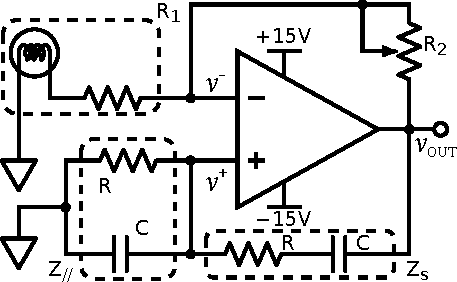
\includegraphics[width=.35\textwidth]{../E08/latex/osc_w_lamp.pdf}
\caption{Schema dell'oscillatore a ponte di Wien con regolazione del guadagno ottenuta mediante una lampadina a filamento.}
\label{cir8:with_lamp}
\end{wrapfigure}

Inizialmente la resistenza sarà più fredda e pertanto il guadagno del circuito sarà maggiore di \num{1}, innescando l'oscillazione.
Con il passaggio di corrente nella lampadina, essa si scalderà e aumenterà la propria resistenza, diminuendo il guadagno portandolo a valori inferiori di \num{1}.
Ciò porterà il circuito a stabilizzarsi con un guadagno unitario e pertanto a generare un'oscillazione di frequenza $f_0$ di ampiezza costante.

Utilizzando un trimmer è possibile aggiustare il valore della resistenza $R_2$ in modo che l'oscillazione autosostenuta del ponte di Wien abbia l'ampiezza desiderata.

$$$$
$$$$

\begin{figure}[htpc]
\centering
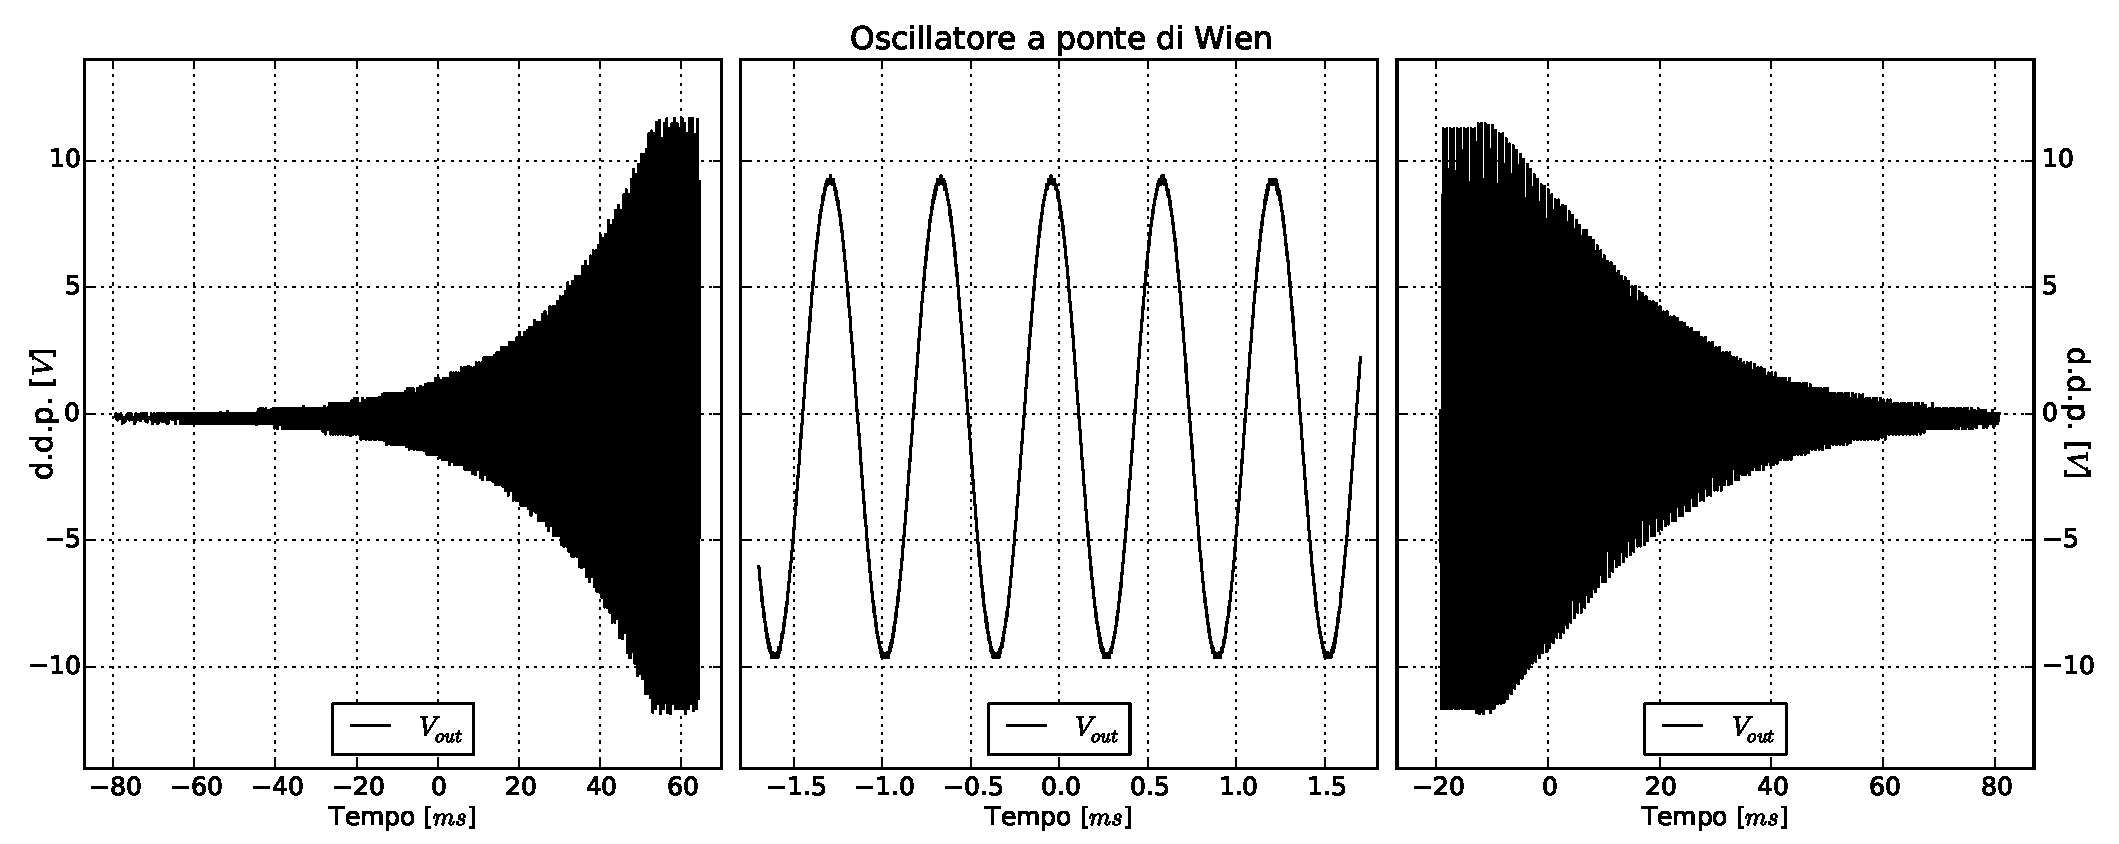
\includegraphics[width=.95\textwidth]{../E08/latex/wien.pdf}
\caption{Risposta del circuito oscillatore, nel grafico a sinistra in guadagno è maggiore di \num{1}, nel grafico centrale il guadagno è stabile, nel grafico a destra il guadagno è inferiore di \num{1}.}
\label{fig8:wien}
\end{figure}

\subsection{Pole-zero compensation di una sonda}

La \textit{pole-zero compensation} è una tecnica che permette di compensare dei poli del sistema. Tale procedimento ci permette di eliminare dipendenze dalla grequenza e di effettuare misure precise di circuiti senza interferenze da parte dell'apparato di misura.

Essa consiste nel posizionare, aggiungendo un'ulteriore parte circuitale, uno zero alla funzione di trasferimento esattamente nel punto in cui esiste un polo .
In equazioni si traduce con:

\[
  \begin{array}{lr}
H(s) = \frac{a(s)}{b(s)} \quad tc \quad b(s_0) = 0 \\
f(s) \quad tc \quad f(s_0) = 0
  \end{array}\left\}
\quad \longrightarrow \quad H'(s) = \frac{a(s)f(s)}{b(s)} \quad tc \quad H'(s_0) = 0
\right.
\]

Per ottenere questo risultato, si antepone all'oscilloscopio una sonda compensata il cui circuito schematizzato è proposto in Figura \ref{cir8:probe}.

\begin{wrapfigure}[13]{r}{0.45\textwidth}
\centering
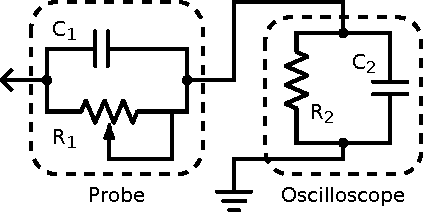
\includegraphics[width=.35\textwidth]{../E08/latex/probe.pdf}
\caption{Schema del circuito di misura composto dall'oscilloscopio e dalla sonda.}
\label{cir8:probe}
\end{wrapfigure}
Come si può notare la sonda e l'oscilloscopio formano un partitore e pertanto la tensione misurata dallo strumento non sarà la stessa del circuito.
Sarà determinata dalla funzione di trasferimento:

\begin{equation}
H(s)=\frac{Z_{osc}}{Z_{probe}+Z_{osc}} = \frac{R_2}{R_1+R_2}\,\frac{1+R_1C_1s}{1+\frac{R_1R_2}{R_1+R_2}(C_1+C_2)s}
\end{equation}

Da questa formula è evidente che la compensazione del polo sia ha quando la seconda frazione è uguale ad \num{1} e quindi il partitore diventa completamente resistivo:
\begin{equation*}
1+R_1C_1s = 1+\frac{R_1R_2}{R_1+R_2}(C_1+C_2)s
\end{equation*}
da cui
\begin{equation}
R_1 = R_2 \frac{C_2}{C_1}
\end{equation}

Questa relazione permette di spostare lo zero della sonda proprio sul polo dell'oscilloscopio permettendone la compensazione.
Dal punto di vista pratico, rendiamo la sonda insensibile alla frequenza e, fissati i parametri $R_2$, $C_2$ e $C_1$, si varia $R_1$ finché l'oscilloscopio non misura la stessa tensione $V_{in}$ ridotta di un fattore $\frac{R_2}{R_1+R_2}$.

\begin{figure}[htpc]
\centering
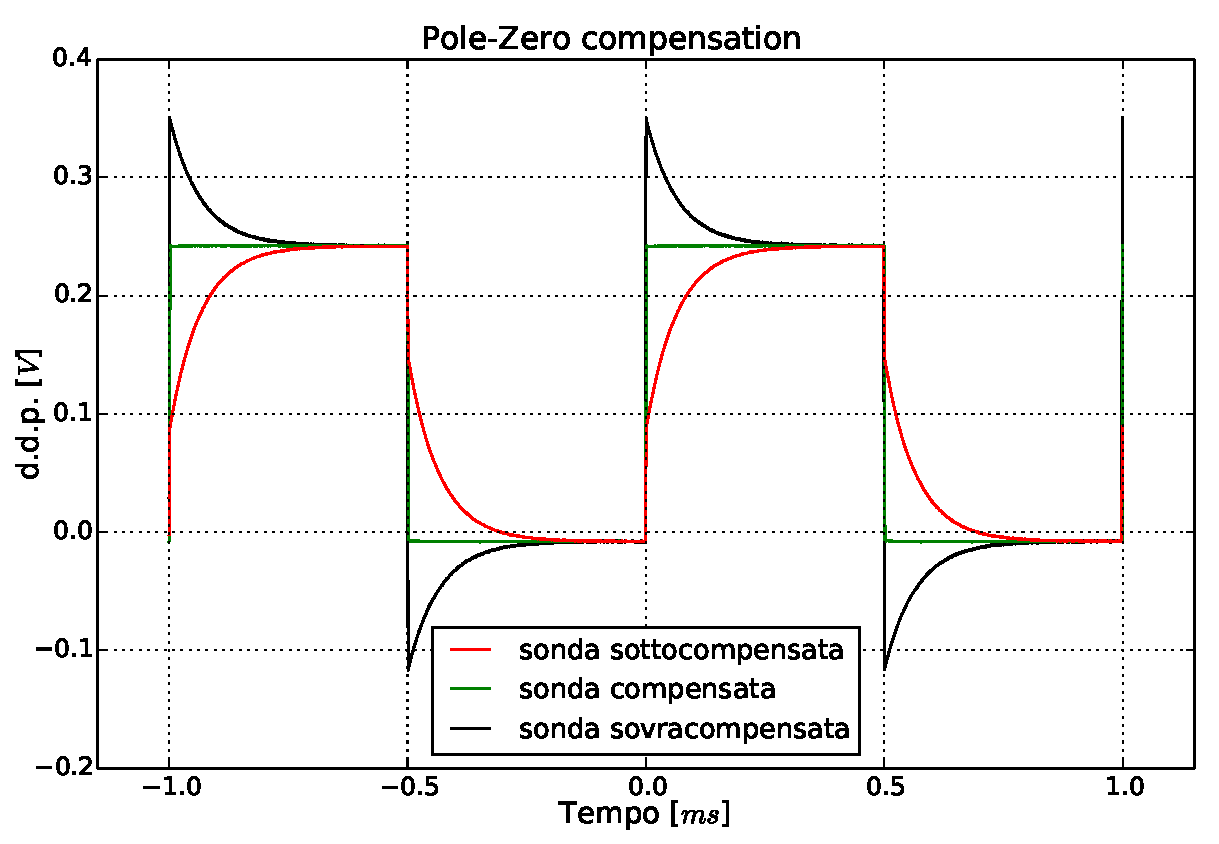
\includegraphics[width=.65\textwidth]{../E08/latex/compensation.pdf}
\caption{Risposta del circuito composto dalla sonda e dall'oscilloscopio visto dall'oscilloscopio stesso. La sonda è stata eccitata con un'onda quadra tramite il generatore interno dell'oscilloscopio.}
\label{fig8:compensation}
\end{figure}

\subsection*{Conclusioni}
In questa esperienza abbiamo costruito un circuito che, come l'oscillatore a rilassamento, fornisce un'oscillazione autosostenuta. La cosa interessandte del ponte di Wien è che la forma d'onda in uscita è praticamente sinusoidale. Ciò può essere utile per applicazioni dove si necessità di una forma d'onda di tale tipo. Nella seconda parte dell'esperienza abbiamo compesato una sonda. Tali sonde sono molto utili per il fatto che sono insensibili alla frequenza del segnale. Se andiamo a rivedere l'Esperienza 3, nel grafico \ref{gr3:slew_rate} vediamo come l'onda quadra in ingresso non sia perfetta. Ciò è dovuto ad un effetto di sovracompensazione della sonda (in quel caso un semplice cavo). Dunque, per esperimenti che riguardano segnali ad alta frequenza o che contengono alte frequenze (onda quadra), è preferibile utilizzare sonde compensate.